% NOVA paper, journal version (Elsevier elsarticle, for Computers & Security; single-anonymized review).
% Build:  latexmk -pdf main.tex
% Tables and figures come from experiments/analysis/paper_results.py, journal_tables.py and split_check.py.
\documentclass[preprint,12pt]{elsarticle}

\usepackage[utf8]{inputenc}
\usepackage[T1]{fontenc}
\usepackage{amsmath,amssymb}
\usepackage{graphicx}
\usepackage{booktabs}
\usepackage{catchfile}
\usepackage{multirow}
\usepackage{makecell}
\usepackage{xcolor}
\usepackage{algorithm}
\usepackage{algpseudocode}
\usepackage{lineno}
\usepackage[hidelinks]{hyperref}
\usepackage[capitalise,noabbrev]{cleveref}

\graphicspath{{../experiments/paper/}}
\newcommand{\results}[1]{../experiments/paper/#1}
\newcommand{\TBD}[1]{\textcolor{red}{[#1]}}
\newcommand{\nova}{\textsc{Nova}}
\newcommand{\unk}{\textsc{unknown}}

% Generated rows are inserted with \CatchFileDef because \input cannot be used inside a tabular.
\newcommand{\resulttable}[4][]{%
\begin{table}[#1]
\centering
\caption{#3 Mean$_{\pm\text{std}}$ over three seeds; best mean in bold. FPR in \%.}
\label{#4}
\small
\setlength{\tabcolsep}{4pt}
\IfFileExists{\results{#2}}{%
\CatchFileDef{\resultrows}{\results{#2}}{}%
\resizebox{\textwidth}{!}{%
\begin{tabular}{@{}lcccccc@{}}
\toprule
Method & OW-F1 & AUT & Det-F1 & FPR & U-AUROC & Forgetting\\
\midrule
\resultrows
\bottomrule
\end{tabular}}}{\TBD{\detokenize{#2} not generated yet}}
\end{table}}

\journal{Computers \& Security}

\begin{document}

\begin{frontmatter}

\title{Open-world adaptation of network intrusion detectors under delayed and scarce labels:
the \nova{} loop and a chronological evaluation on three datasets}

\author[a]{\TBD{Author name}\corref{cor1}}
\ead{author.email@example.com}
\cortext[cor1]{Corresponding author.}
\affiliation[a]{organization={\TBD{Department of Computer Science and Engineering, Green University of Bangladesh}},
            city={Dhaka},
            country={Bangladesh}}

\begin{abstract}
Network intrusion detectors are evaluated on random splits and reach near-perfect scores. In deployment, they
meet drifting traffic and attack classes that did not exist at training time, while analysts can label only a
small fraction of the flows, and only after a delay. Chronological replays of
CIC-IDS2017, CSE-CIC-IDS2018 and UNSW-NB15 give every method the same label budget and delay, and we score them
with metrics that stay comparable when methods learn different classes. We propose \nova{}, an adaptation loop
that rejects unfamiliar flows with a class-conditional $k$-nearest-neighbour detector and recalibrates it for
newly learned classes. It spends the label budget on novel, diverse traffic, propagates analyst labels to
agreeing neighbours, keeps rare attacks in a class-balanced memory, and deploys an update or a rollback only
after a hold-out and a forgetting check. We compare \nova{} with eight methods, including re-implementations of
INSOMNIA, NetGuard and class-balanced replay. At a 10\% budget it matches the strongest
baseline on open-world macro-F1 on the CIC datasets (0.752 against 0.755 and 0.738 against 0.730) and flags significantly fewer benign flows
on all three datasets. With 1\% of CIC-IDS2017 labelled, it leads by 8.5 points. On UNSW-NB15, stale
rejection thresholds push the replay-based methods far below the never-updated model; an ablation shows that
\nova{}'s per-class recalibration avoids this. We also report where it fails: short-lived attacks that resemble benign
traffic, a neural classifier, and one dataset at the smallest budget. Code,
configurations and per-flow predictions are released.
\end{abstract}

\begin{keyword}
network intrusion detection \sep concept drift \sep open-set recognition \sep active learning \sep
continual learning \sep evaluation methodology
\end{keyword}


\end{frontmatter}

\section{Introduction}
\label{sec:intro}

Machine-learning network intrusion detection systems (NIDS) classify network flows as benign or as one of several
attack classes. On public benchmarks such as CIC-IDS2017~\cite{sharafaldin2018} they routinely report accuracies
above 99\%. Most of these results come from random train/test splits, in which flows of the same attack session
fall on both sides of the split, so the test asks whether the model recognises traffic it has effectively already
seen. Network traffic is time-dependent, and estimates obtained with a chronological split differ from those of a
random split~\cite{nismara2026temporal}. Careful sequence evaluations find that the evaluation protocol matters far
more than the model architecture~\cite{moczkodan2026transformers}. These are instances of the temporal and spatial
biases described for security classifiers in general~\cite{pendlebury2019tesseract,arp2022dos}.
\Cref{sec:res-split} quantifies the gap on our data. The same gradient-boosting classifier reaches 99.8\%
accuracy on a random split of CIC-IDS2017, the figure usually reported. Trained on the first 30\% of the capture
and tested on the rest, it reaches 72.6\%, and its macro-F1 falls from 0.761 to 0.125, because eleven of the
classes in the test period never occur in training.

A deployed detector faces four conditions that random splits hide. First, \emph{new attack classes} appear after
training. A closed-set model assigns them to some known class, most often to benign traffic, and nothing tells
the operator that it is guessing. Second, \emph{labels are scarce}: an analyst can inspect only a small fraction of
the flows. Third, \emph{labels are late}: ground truth for today's traffic arrives after today's decisions were
made. Fourth, every model update is a \emph{deployment}, and a bad update degrades detection silently unless
something checks it. Prior work addresses these conditions one at a time (\cref{sec:related}). Drift
detectors~\cite{jordaney2017transcend,yang2021cade} flag drifting samples but do not adapt. Adaptive
NIDS~\cite{andresini2021insomnia,zhang2024aoc,zhang2025ssf} update mostly binary detectors, often from their own
pseudo-labels, and rarely model label delay. Active-learning methods~\cite{chen2023continuous,gupta2025netguard}
choose which samples to label but assume a closed set of classes. Open-set NIDS~\cite{zhang2020osr,corsini2023ood}
reject unknown traffic, but only on static splits.

This article studies the four conditions together and asks five research questions:
\begin{description}
  \item[RQ1] How large is the gap between random-split and chronological evaluation for the same classifier?
  \item[RQ2] Under one label budget and delay, which adaptation strategy keeps a multi-class open-world detector
        most accurate, and at what false-positive cost?
  \item[RQ3] How do the strategies behave when labels become ten times scarcer?
  \item[RQ4] Which components of the proposed method matter, and do their effects carry over to datasets that were
        not used for its design?
  \item[RQ5] How sensitive are the conclusions to the label delay, the rejection thresholds and the classifier?
\end{description}

\textbf{Contributions.}
\begin{enumerate}
  \item An evaluation protocol for drift-aware open-world NIDS: chronological replay in windows, a label oracle
        that enforces the same budget and delay for every method, and metrics that stay comparable when methods
        learn different classes (\cref{sec:problem}). We show a property of open-world scoring that matters in
        practice: a method that never learns a new class can outscore one that learns it imperfectly
        (\cref{sec:res-budget}).
  \item \nova{} (Novelty-aware, Open-world, Validated Adaptation), which combines class-conditional $k$-NN
        rejection with per-class recalibration, a novelty-weighted and cluster-diverse query, agreement-checked
        label propagation, a benign-weighted class-balanced memory, and a deployment guard with rollback
        (\cref{sec:method}).
  \item A comparison with eight methods, including re-implementations of four published approaches, on three
        datasets from two laboratories, with all design decisions made on one development dataset and the other
        two used only for evaluation (\cref{sec:setup,sec:results}).
  \item Analyses that explain the results: a full ablation on all three datasets, per-class results, sensitivity
        to label delay, rejection thresholds and classifier, and an offline test of whether a meta-learned
        representation would help (\cref{sec:results}).
  \item An open-source research console that stores the configuration, data hash and per-flow decision of every
        run, so that each number in this article can be reproduced.
\end{enumerate}

\textbf{Relation to our conference paper.} \TBD{A preliminary version of this work appears in [conference
reference]. This article adds the random-versus-chronological comparison (RQ1), a dataset audit, per-window
confidence intervals and per-class explanations for the ablations, the metric decomposition and guard statistics,
the label-delay, threshold and classifier sensitivity studies, per-class and failure analyses, the
representation-learning probe, an extended related-work survey and a full description of the protocol and
method.}

\section{Background and related work}
\label{sec:related}

\Cref{tab:families} groups prior work into five lines of research and lists the properties that matter in our
setting. No line covers all of them; \nova{} borrows one element from each.

\begin{table}[t]
\centering
\caption{Lines of prior work and the properties they typically address (\checkmark: usually addressed;
$\circ$: partly or in some works; --: usually not addressed).}
\label{tab:families}
\small
\resizebox{\textwidth}{!}{%
\begin{tabular}{@{}lcccccc@{}}
\toprule
Line of work & \makecell{Rejects\\unknown flows} & \makecell{Adapts\\the model} & \makecell{Uses analyst\\labels} &
\makecell{Models label\\delay} & \makecell{Validates\\updates} & \makecell{Multi-class\\attacks} \\
\midrule
Drift detection and rejection~\cite{jordaney2017transcend,barbero2022transcending,yang2021cade,han2023owad}
  & \checkmark & $\circ$ & $\circ$ & -- & -- & $\circ$ \\
Self-training adaptive NIDS~\cite{andresini2021insomnia,zhang2024aoc,zhang2025ssf,mousavipour2025shift}
  & -- & \checkmark & $\circ$ & -- & -- & -- \\
Active learning under drift~\cite{chen2023continuous,gupta2025netguard,prabhu2021clue}
  & -- & \checkmark & \checkmark & -- & -- & $\circ$ \\
Continual learning with replay~\cite{amalapuram2023augmented,amalapuram2024soul,chrysakis2020online}
  & $\circ$ & \checkmark & $\circ$ & -- & -- & $\circ$ \\
Open-set NIDS~\cite{zhang2020osr,corsini2023ood}
  & \checkmark & -- & -- & -- & -- & \checkmark \\
\midrule
\nova{} (this work) & \checkmark & \checkmark & \checkmark & \checkmark & \checkmark & \checkmark \\
\bottomrule
\end{tabular}}
\end{table}

\subsection{Evaluation methodology and datasets}
TESSERACT~\cite{pendlebury2019tesseract} showed that two biases inflate results of security classifiers:
\emph{spatial} bias, when the class ratio of the test set is unrealistic, and \emph{temporal} bias, when training
data postdate test data. It proposed time-consistent splits and the area-under-time (AUT) metric, which we adopt.
Arp et al.~\cite{arp2022dos} catalogue ten pitfalls of machine learning in security, among them data snooping,
inappropriate baselines and lab-only evaluation; our protocol is designed against them (\cref{sec:problem}).

CIC-IDS2017~\cite{sharafaldin2018} and CSE-CIC-IDS2018 are the most widely used flow datasets, and both contain
errors. Engelen et al.~\cite{engelen2021troubleshooting} found feature-extraction artefacts and mislabelled flows
in CIC-IDS2017. Lanvin et al.~\cite{lanvin2022errors} independently found unlabelled attack traffic and showed
that the corrections change reported detection results. Liu et al.~\cite{liu2022error} audited both CIC
datasets. UNSW-NB15~\cite{moustafa2015unsw} was captured on two days with a different tool chain. We use the
three datasets as published and discuss the consequences of their errors in \cref{sec:discussion}. Performance
estimates from chronological splits of these datasets differ from those of random
splits~\cite{nismara2026temporal}, and a recent sequence study on CIC-IDS2017 found that the protocol matters far
more than the model architecture~\cite{moczkodan2026transformers}.

\subsection{Drift detection and rejection}
Transcend~\cite{jordaney2017transcend} attaches conformal credibility scores to the predictions of any classifier
and rejects low-credibility ones as drifting; its successor~\cite{barbero2022transcending} makes the calibration
cheaper. CADE~\cite{yang2021cade} trains a contrastive autoencoder and flags samples whose distance to every class
centroid, scaled by the class's spread, is large; it also explains which features cause the drift. OWAD~\cite{han2023owad}
targets anomaly detectors trained on benign traffic: it calibrates their outputs, detects normality shift with a
permutation test, selects a few samples that explain the shift for labelling, and adapts with a regulariser
against forgetting. These works decide \emph{whether} the input distribution has moved. \nova{} uses a
rejection rule of the same kind, but conditions it on the predicted class (a single centroid cannot represent
multi-modal benign traffic, \cref{sec:res-ablation}) and couples it with labelling and deployment decisions.

\subsection{Adaptive network intrusion detection}
INSOMNIA~\cite{andresini2021insomnia} retrains a binary detector on drifting CIC-IDS2017 traffic. In every window,
the least-confident flows are labelled by a nearest-centroid estimator instead of an analyst, and both models are
fine-tuned. Because the estimator can only produce classes seen in training, genuinely new attacks are never
learned, and its errors are fed back into training. AOC-IDS~\cite{zhang2024aoc} fine-tunes a contrastive
autoencoder online on pseudo-labels from a Gaussian fit of similarity to a benign prototype. SSF~\cite{zhang2025ssf}
adds drift detection, a learned selection of old and new samples, a small labelled share and strategic forgetting.
Mousavipour et al.~\cite{mousavipour2025shift} detect shift at the distribution level, explain it with masks and
adapt with relational distillation. ENIDrift~\cite{wang2022enidrift} keeps an ensemble of sub-classifiers over
incremental packet embeddings and prunes unstable members. Most of these methods are binary, rely on their own
pseudo-labels, and were evaluated on random or day-wise splits without label delay. We re-implement INSOMNIA as a
representative of the self-training line.

\subsection{Active learning under drift}
Chen et al.~\cite{chen2023continuous} retrain an Android-malware classifier monthly and choose samples to label
with a pseudo-loss computed from nearest training neighbours in a hierarchically contrastive embedding; they show
that similarity-based selection beats plain uncertainty under drift. NetGuard~\cite{gupta2025netguard} adapts a
NIDS from CIC-IDS2017 to CSE-CIC-IDS2018: it labels the flows with the highest density ratio between new and
labelled traffic (Gaussian mixtures on each) and synthesises rare attacks with a tabular generator.
CLUE~\cite{prabhu2021clue} clusters uncertainty-weighted embeddings and labels the sample nearest each centroid,
which yields uncertain and diverse picks. \nova{}'s query belongs to this family, but it weights clusters by an
open-world novelty score, keeps a uniform share for benign drift, and runs every window under a label delay. We
re-implement uncertainty sampling and NetGuard's selection.

\subsection{Continual learning with replay}
Continual learning keeps a memory of past samples to avoid forgetting. Class-balancing reservoir sampling
(CBRS)~\cite{chrysakis2020online} lets rare classes survive in a fixed memory. Amalapuram et
al.~\cite{amalapuram2023augmented} extend it for intrusion detection and make interference-aware retrieval
cheaper; SOUL~\cite{amalapuram2024soul} adds semi-supervised label generation for unseen tasks, keeping a
pseudo-label only if it agrees with a similarity vote over the memory. We re-implement CBRS replay, which turned
out to be the strongest baseline, and \nova{}'s label propagation follows SOUL's agreement principle.

\subsection{Open-set recognition and out-of-distribution detection}
Open-CNN~\cite{zhang2020osr} fits a Weibull distribution to the activations of known classes and estimates an
unknown-class probability. Corsini and Yang~\cite{corsini2023ood} compare out-of-distribution detectors on the CIC
datasets and find the distance to the $k$-th nearest training embedding the strongest single detector, in line
with deep $k$-NN results in vision~\cite{sun2022knn}. These detectors were evaluated on static splits.
\nova{} uses a class-conditional $k$-NN detector and recalibrates it whenever a new class is learned; we show
that the recalibration is what keeps learned classes from being rejected after drift (\cref{sec:res-main}).
Few-shot open-set recognition~\cite{liu2020peeler} learns embeddings by episodic meta-learning; we test whether
such an embedding would help in \cref{sec:res-meta}.

\section{Problem setting, protocol and metrics}
\label{sec:problem}

\subsection{Stream, decisions and labels}
Flows $(x_t, y_t)$ arrive in timestamp order, where $x_t \in \mathbb{R}^d$ are flow features and $y_t \in
\mathcal{C}$ is the flow's class (benign or an attack type). A model is trained on an initial period whose
classes $\mathcal{C}_0 \subset \mathcal{C}$ are known. The rest of the stream is processed in consecutive windows
$W_1, W_2, \dots$ of $n$ flows.

For each flow, the deployed model $f$ outputs either a class it knows or \unk{}. We give \unk{} a precise
operational meaning: ``unfamiliar to this model, send to an analyst''. It is neither an alarm nor a statement
that the flow is malicious. A deployed NIDS has to make this distinction, because benign traffic that the model
has never seen should be reviewed, not blocked.

After predicting window $W_w$, a method may request ground truth for at most $B \cdot n$ of its flows (the label
\emph{budget} $B$). The labels arrive at window $w + \delta$ (the label \emph{delay} $\delta$). A label oracle is
the only path to ground truth: it enforces the budget and the delay, refuses a second request for the same
window, and counts every label it hands out. Methods that do not choose which flows to label receive a uniform
random sample of the budget, so every method that uses labels receives exactly the same number. A method may
replace the deployed model after any window; the new model only affects later windows.

\subsection{Integrity rules}
The protocol enforces the following rules in code and records them in every run:
\begin{enumerate}
  \item \emph{No look-ahead.} Preprocessing statistics (log transform and standardisation) are fitted on the
        training period only; the stream is never used to fit anything before it is predicted.
  \item \emph{Fixed reference set.} The last 20\% of the training period is held out as a reference set. It is
        used to calibrate the initial rejection thresholds and to measure forgetting. It keeps only classes that
        occur in the fitted part of the training period: a class that first appears in the reference period
        (SSH-Patator in CIC-IDS2017) was never learned, and keeping it would turn ``forgetting'' into a measure of
        unknown-attack detection.
  \item \emph{One labelling path.} Strategies obtain labels only through the oracle, with the same budget and
        delay.
  \item \emph{Development and held-out data.} All design decisions are made on one dataset; the others are used
        only with the frozen configuration (\cref{sec:setup}).
\end{enumerate}

\subsection{Metrics}
\label{sec:metrics}
Let $\hat{y}_t$ be the decision for flow $t$ and $K_t$ the set of classes known to the model that scored it.
Standard open-set macro-F1 maps every flow of an unknown class to a single \unk{} label. Two methods that learn
different classes are then scored on different label sets, and their scores cannot be compared. We therefore use
a fixed class set.

\textbf{Open-world macro-F1 (OW-F1).} A decision is credited as correct if
\begin{equation}
\label{eq:owcredit}
\text{correct}_t = \bigl[\hat{y}_t = y_t\bigr] \;\lor\; \bigl[y_t \notin K_t \land \hat{y}_t = \unk{}\bigr],
\end{equation}
that is, if it names the true class, or if the true class is unknown to the deployed model and the decision is
\unk{}. Per-class precision and recall are computed over the fixed set $\mathcal{C}$ of all true classes in the
stream, with credited \unk{} decisions counted as the true class, and OW-F1 is their unweighted mean.

Equation~\eqref{eq:owcredit} has a property that matters when reading the results. The credit for \unk{} lasts
only while a class is unknown. A method that never learns a new class and keeps rejecting it is credited in full
for that class. A method that learns the class imperfectly is scored on its class-level F1, which can be lower. We
report this deliberately: rejecting an attack the system cannot name is a safe outcome for an operator, but it
also means that OW-F1 alone cannot distinguish ``learned nothing'' from ``learned well''. We therefore always
read it together with the binary detection metrics and the per-class results (\cref{sec:res-budget,sec:res-perclass}).

\textbf{AUT.} The area under the per-window OW-F1 curve, normalised to $[0,1]$~\cite{pendlebury2019tesseract}:
\begin{equation}
\mathrm{AUT} = \frac{1}{N-1} \sum_{w=1}^{N-1} \frac{F_w + F_{w+1}}{2},
\end{equation}
where $F_w$ is the OW-F1 of window $w$ and $N$ the number of windows. AUT weights every window equally, whereas
the pooled OW-F1 weights every class equally over the whole stream; a short-lived class therefore moves OW-F1 much
more than AUT.

\textbf{Binary detection.} A flow is \emph{flagged} when its decision is not benign, i.e.\ an attack class or
\unk{}; both reach an analyst. Detection F1, recall and false-positive rate (FPR, the share of benign flows that
are flagged) are comparable with binary NIDS work, and FPR is the analyst's review load from benign traffic.

\textbf{Unknown AUROC.} How well the open-world score $s(x)$ (\cref{sec:unknown}) ranks flows of classes unknown
to the deployed model above flows of known classes, independently of the threshold.

\textbf{Forgetting.} The largest drop of macro-F1 on the reference set below its running maximum over the
stream, i.e.\ $\max_w \bigl(\max_{v \le w} R_v - R_w\bigr)$ where $R_w$ is the reference macro-F1 of the model
deployed after window $w$.

We also report labels used and training time. Every metric is computed per window and on the pooled stream; tables
report pooled values with the mean and standard deviation over three seeds.

\section{\nova{}}
\label{sec:method}

\nova{} wraps any probabilistic classifier $f$; we use gradient-boosted trees. It maintains three pieces of
state: a training memory $M$ of labelled flows, a calibration store $Q$ of held-out analyst labels that are never
used for training, and the previously deployed model $f_{\text{prev}}$. \Cref{alg:nova} gives the loop that runs
after every window. Each component addresses one of the four conditions of \cref{sec:intro}:
\begin{itemize}
  \item new classes: open-world scoring with per-class recalibration;
  \item scarce labels: the query and label propagation;
  \item late labels: the memory;
  \item silent degradation: the deployment guard and rollback.
\end{itemize}
\Cref{tab:hyper} lists the hyper-parameters.

\begin{algorithm}[t]
\caption{\nova{} after window $W_w$ has been predicted}
\label{alg:nova}
\begin{algorithmic}[1]
\Require deployed model $f$, previous model $f_{\text{prev}}$, memory $M$, calibration store $Q$
\State $s \gets$ unknown scores of $W_w$ under $f$ \Comment{\cref{sec:unknown}}
\State request labels for $\textsc{Query}(W_w, s, Bn)$; they arrive at window $w{+}\delta$ \Comment{\cref{sec:query}}
\State $L \gets$ analyst labels that arrived now
\If{$f$ was deployed within the last two windows \textbf{and} $\mathrm{F1}_L(f_{\text{prev}}) - \mathrm{F1}_L(f) > \rho$ \textbf{and} $\mathrm{F1}_{\text{ref}}(f) - \mathrm{F1}_{\text{ref}}(f_{\text{prev}}) \le \epsilon$}
   \State roll back to $f_{\text{prev}}$ \Comment{\cref{sec:guard}}
\EndIf
\State $H \gets$ stratified hold-out of $L$ (share $h$); \ $T \gets L\setminus H$
\State $P \gets \textsc{Propagate}(T)$ \Comment{\cref{sec:prop}}
\State $f' \gets \textsc{Train}(M \cup T \cup P)$ with weight $\omega$ on $T \cup P$; calibrate on reference $\cup\; Q$
\If{$\mathrm{F1}_H(f') \ge \mathrm{F1}_H(f)$ \textbf{and} $\mathrm{F1}_{\text{ref}}(f) - \mathrm{F1}_{\text{ref}}(f') \le \epsilon$}
   \State deploy $f'$; $f_{\text{prev}} \gets f$
\EndIf
\State move flows of $H$ to $Q$ if their class has room and $\ge q_{\min}$ flows in $M$, otherwise to $M$
\State $M \gets \textsc{CBRS}(M, T \cup P)$ \Comment{\cref{sec:memory}}
\end{algorithmic}
\end{algorithm}

\subsection{Open-world scoring and recalibration}
\label{sec:unknown}
For a flow $x$ with predicted class $c = \arg\max_j p_j(x)$, \nova{} computes two scores, each normalised so that
its decision threshold is 1:
\begin{equation}
s_{\text{msp}}(x) = \frac{1 - p_c(x)}{1 - \tau^{\text{msp}}_c}, \qquad
s_{\text{knn}}(x) = \frac{d_k\!\left(x, \mathcal{B}_c\right)}{\tau^{\text{knn}}_c},
\end{equation}
where $p_c(x)$ is the maximum softmax probability and $d_k(x,\mathcal{B}_c)$ the Euclidean distance from $x$ to
its $k$-th nearest neighbour in a bank $\mathcal{B}_c$ of up to 3{,}000 training flows of class $c$. The unknown
score is $s(x) = \max\bigl(s_{\text{msp}}(x), s_{\text{knn}}(x)\bigr)$, and the decision is \unk{} if and only if
$s(x) > 1$. The same score ranks flows for the unknown AUROC and drives the query.

\textbf{Per-class thresholds.} A single global threshold is dominated by the majority class: it either rejects
most flows of a newly learned, still sparse class, or accepts everything. \nova{} therefore calibrates one pair
of thresholds per class on held-out flows that the classifier did not train on. $\tau^{\text{msp}}_c$ is the 2\%
quantile of the confidence of held-out flows predicted as $c$; a class with fewer than 20 such flows receives the
most lenient threshold of the other classes. $\tau^{\text{knn}}_c$ is the 99\% quantile of $d_k$ over held-out
flows that belong to $c$ and are predicted as $c$; with fewer than 30 such flows, it falls back to a leave-one-out
estimate on the bank itself.

\textbf{Class-conditional neighbours.} The neighbour search is restricted to the bank of the \emph{predicted}
class. Benign traffic consists of many protocol and application modes, which a single class centroid, as in
CADE~\cite{yang2021cade}, cannot represent: the centroid lies between the modes, and every mode looks distant. A
$k$-NN distance follows each mode. Conditioning on the predicted class also makes the score answer the operational
question, ``is this flow typical of what the model says it is?''.

\textbf{Recalibration.} Thresholds are recomputed for every candidate model on the reference set plus the
calibration store $Q$. Without $Q$, a class that drifts after training keeps thresholds fitted on training-period
traffic. Its later flows are then rejected even after the model has learned the class. This is the mechanism that
pulls the replay baselines below the static model on UNSW-NB15 (\cref{sec:res-main}).

\subsection{Query}
\label{sec:query}
Of the budget $Bn$ labels for a window, a share $\rho_u$ is drawn uniformly at random. This keeps an unbiased
view of benign drift, which a purely novelty-driven query would ignore. The remaining labels are spread over $K$
$k$-means clusters of the window's flows. Cluster $j$ receives at least one label and a quota proportional to
\begin{equation}
q_j \propto \sqrt{|j|}\,\bigl(0.1 + \bar{s}_j\bigr),
\end{equation}
where $|j|$ is the cluster size and $\bar{s}_j$ the mean unknown score of its flows, clipped to $[0,5]$. Inside a
cluster, the flows with the highest unknown score are chosen first.

The square root damps size: a large benign mode still receives labels, but not in proportion to its volume.
The novelty term sends labels to compact clusters of unfamiliar flows, which is how an emerging attack looks in a
window. The constant 0.1 keeps familiar clusters from receiving no labels at all.

\subsection{Label propagation}
\label{sec:prop}
Each analyst label is extended to nearby unlabelled flows of the same window under two agreement conditions. An
unlabelled flow $u$ takes class $c$ when
\begin{enumerate}
  \item its $\min(k_p, n_c)$ nearest labelled flows all have class $c$, where $n_c$ is the number of labels of
        $c$ in the window, and
  \item its distance to the nearest labelled flow is within the radius of $c$, the 90th percentile of
        nearest-same-class distances among the labels of $c$.
\end{enumerate}
At most $r$ propagated labels are kept per analyst label of $c$, closest first, and a class with a single label
does not spread. Unlike self-training~\cite{andresini2021insomnia,zhang2024aoc}, propagation never uses the model's
own predictions and never creates a class; it follows the agreement principle of SOUL~\cite{amalapuram2024soul}.
Hold-out flows are never propagated, so the guard is not evaluated on copies of its own training data.

\subsection{Memory}
\label{sec:memory}
The training memory holds 20{,}000 flows and is a class-balancing reservoir~\cite{chrysakis2020online}. It is
initialised by streaming the training period through the reservoir. When it is full, a new flow of a class that is not the largest evicts
a random flow of the currently largest class, and a flow of the largest class replaces a random member of its
own class with reservoir probability. ``Largest'' compares class size divided by a class weight. Benign traffic
receives weight $\beta$, so it may occupy $\beta$ times the share of any attack class. Benign traffic is
multi-modal, and starving it raises false alarms. The newest labels receive training weight $\omega$, so that a
model update reflects what has just been observed.

\subsection{Deployment guard and rollback}
\label{sec:guard}
Every candidate is trained on the memory plus the new labels, minus a stratified hold-out $H$ of the newest
analyst labels: a share $h$ of each class with at least four labels. The candidate is deployed only if two
conditions hold:
\begin{enumerate}
  \item it is at least as good as the deployed model on $H$;
  \item it loses at most $\epsilon$ macro-F1 on the reference set.
\end{enumerate}
Both comparisons use the open-world credit of \cref{eq:owcredit}, so models that know different classes are
compared on the same task. They ignore classes with fewer than $m$ labels in the compared slice: a class with one
labelled flow makes macro-F1 jump by $1/|\mathcal{C}|$ on a single decision.

After a deployment, the next two label batches are also used to check the new model against its predecessor. If
the predecessor is better by more than $\rho$, \nova{} rolls back. A rollback is itself a deployment and must pass
the same reference check. In our development runs, an unchecked rollback once restored an early model that did not
know most of the attack classes learned since, and undid what the stream had taught.

\subsection{Hyper-parameters and cost}
\Cref{tab:hyper} lists all hyper-parameters. They were set from the design arguments above, checked in two
development runs on CIC-IDS2017, and then frozen for every experiment on every dataset.

Per window, \nova{} performs one $k$-NN scoring pass, one $k$-means run on 4{,}000 flows, and at most one candidate
training on about 20{,}000 flows. The scoring pass uses chunked matrix products against banks of at most 3{,}000
flows per class. Training dominates the cost: \nova{} spends 13--14 minutes of training per 70-window run, 1.2 to 2.2
times as much as CBRS replay (\cref{sec:res-cost}).

\begin{table}[t]
\centering
\caption{\nova{} hyper-parameters (frozen after development on CIC-IDS2017).}
\label{tab:hyper}
\small
\begin{tabular}{@{}llp{0.55\textwidth}@{}}
\toprule
Symbol & Value & Role \\
\midrule
$k$ & 10 & neighbour rank of the $k$-NN score; bank of 3{,}000 flows per class \\
-- & 2\%, 99\% & quantiles for $\tau^{\text{msp}}_c$ and $\tau^{\text{knn}}_c$ \\
$\rho_u$ & 0.2 & uniformly sampled share of the label budget \\
$K$ & 24 & $k$-means clusters for the query \\
$k_p$, $r$ & 5, 5 & propagation agreement size; propagated labels per analyst label \\
$\beta$ & 4 & benign weight in the class-balanced memory (capacity 20{,}000) \\
$\omega$ & 2 & training weight of the newest labels \\
$h$ & 25\% & hold-out share of new analyst labels for the guard \\
$|Q_c|$, $q_{\min}$ & 200, 50 & calibration flows per class; memory flows required before a class feeds $Q$ \\
$\epsilon$ & 0.05 & tolerated reference macro-F1 loss \\
$\rho$ & 0.05 & rollback margin (two-window watch) \\
$m$ & 5 & minimum labels per class in guard comparisons \\
\bottomrule
\end{tabular}
\end{table}

\section{Experimental setup}
\label{sec:setup}

\subsection{Datasets}
\Cref{tab:datasets} summarises the three datasets. Each is replayed in timestamp order. From each we take 400{,}000
flows evenly spaced over time, deterministically, so that every method and seed sees the same data. The first
30\% form the training period. The last 20\% of the training period is the reference set (\cref{sec:problem}),
and the remaining 280{,}000 flows form 70 windows of 4{,}000 flows. Rows without a valid timestamp or label are
skipped when reading.

\textbf{CIC-IDS2017}~\cite{sharafaldin2018} covers five working days of a testbed network. We use the
\texttt{TrafficLabelling} CSVs, the variant that keeps timestamps; their afternoon times are written without
AM/PM, and we restore them from the capture schedule. The training period (Monday and Tuesday morning) contains
only benign traffic and FTP-Patator, so every attack in the stream is new.

\textbf{CSE-CIC-IDS2018} covers ten days with a larger network and attack set. We use the ``Processed Traffic
Data for ML'' CSVs, thinned to one row in eight per file before sampling to keep the replay tractable. Seven
attack classes occur in the training period and seven appear later. Several day files of the published CSVs are
truncated at 1{,}048{,}575 rows, a spreadsheet limit, which we leave as is.

\textbf{UNSW-NB15}~\cite{moustafa2015unsw} was captured on two days, about four weeks apart, with a different
tool chain. Every class already occurs on the first day, so no class would be new in a chronological replay. As is
common in open-set NIDS work, we remove four attack classes (DoS, Reconnaissance, Shellcode and Worms) from the
training period. They appear in the stream as unknown attacks. The other classes are known, but their February
traffic differs from the January training traffic.

\begin{table}[t]
\centering
\caption{Datasets (after replay sampling: 400k flows, 70 windows of 4{,}000 flows).}
\label{tab:datasets}
\small
\begin{tabular}{@{}lccc@{}}
\toprule
 & CIC-IDS2017 & CSE-CIC-IDS2018 & UNSW-NB15 \\
\midrule
Source flows & 2.83\,M & 16.2\,M & 2.54\,M \\
Days covered & 5 & 10 & 2 \\
Classes (incl.\ benign) & 15 & 15 & 10 \\
Attack classes in training & 1 & 7 & 5 \\
New in stream & 12 & 7 & 4 (held out) \\
Model input features & 79 & 78 & 97 \\
\bottomrule
\end{tabular}
\end{table}

\textbf{Preprocessing.} Identifier columns (flow ID, source and destination address, source port, timestamps;
for UNSW-NB15 also the destination port) are dropped, so the model cannot memorise hosts. Non-finite values are replaced by the training-period median.
Numeric features are transformed with $\operatorname{sign}(v)\log(1+|v|)$ to tame heavy tails, then standardised
with training-period statistics. Categorical fields (UNSW-NB15's protocol, state and service) are one-hot encoded
with an ``unseen'' bucket. Nothing is fitted on the stream.

\subsection{Label regime and classifier}
The main budget is $B = 10\%$ of each window (400 labels), and the low budget $B = 1\%$ (40 labels). The delay is
$\delta = 1$ window, and \cref{sec:res-sens} varies it. Every method that uses labels receives exactly the same
number; INSOMNIA uses none by design.

All methods use the same classifier, scikit-learn's histogram gradient boosting with 150 iterations and L2
regularisation 1.0. Classes with fewer than five labelled flows are left out of training and stay \unk{}. All
methods also use the same open-world detector (\cref{sec:unknown}), except in the detector ablation. The
differences between methods therefore come from the adaptation strategy alone. \Cref{sec:res-sens} repeats the
main comparison with a two-layer MLP.

\subsection{Baselines}
\label{sec:baselines}
We compare with four generic strategies and four methods re-implemented from the literature. All replay memories
hold 20{,}000 flows and are initialised from the training period.
\begin{description}
  \item[Static.] The initial model, never updated: the lower bound.
  \item[Periodic retrain.] From scratch every five windows, on the training data plus the last five labelled
        windows; always deployed.
  \item[Continual replay.] A uniform reservoir memory; retrained whenever labels arrive; always deployed.
  \item[Guarded selective.] Retrained only when a drift detector (Kolmogorov--Smirnov test, population stability
        index or mean-confidence drop) fires or the \unk{} rate exceeds 15\%. The newest labelled window is used as
        a hold-out, the candidate must pass the same gain and forgetting checks as in \nova{}, and a deployed model
        can be rolled back. It shows what a guard achieves without \nova{}'s other components.
  \item[Uncertainty sampling.] Least-confidence active learning on top of continual replay. It is the standard
        query baseline of the active-learning works above and INSOMNIA's ``uncertainty sampling + oracle'' upper
        bound~\cite{andresini2021insomnia}.
  \item[INSOMNIA]~\cite{andresini2021insomnia}, multi-class: after each window, the least-confident 50\% of its
        flows are labelled by a nearest-centroid estimator and added to a pseudo-labelled memory; no analyst
        labels are used.
  \item[NetGuard PS]~\cite{gupta2025netguard}: NetGuard's density-aware prior selection, with one diagonal
        Gaussian mixture (up to eight components) on the labelled memory and one on the new window. The flows with
        the largest log-density ratio are labelled. The generative minority augmentation, which needs GPU hours
        per cycle, is not reproduced.
  \item[CBRS replay]~\cite{chrysakis2020online,amalapuram2023augmented}: the class-balancing reservoir memory used
        for NIDS replay, with uniformly sampled labels, retrained whenever labels arrive.
\end{description}

\subsection{Development and held-out data}
All design decisions, including the components of \nova{}, its hyper-parameters and the CIC-IDS2017 ablation,
were made on CIC-IDS2017. CSE-CIC-IDS2018 and UNSW-NB15 were not used for any design decision. We only checked
their class composition with one run of the static model, which revealed that no UNSW-NB15 class is new without a
hold-out. Both datasets are evaluated with the configuration frozen on CIC-IDS2017. The analyses that we ran on
them after the main results (the ablations and the low budget) change nothing in the method; we mark them as such.

\subsection{Experiments, statistics and implementation}
\Cref{tab:experiments} maps the experiments to the research questions. Each configuration runs with three seeds;
the seed changes model initialisation, label sampling and clustering, not the data. We report the mean and
standard deviation over seeds. To compare \nova{} with another method, we take the per-window difference of their
seed-averaged OW-F1 (or false-positive rate) and report its mean with a 95\% moving-block bootstrap
interval~\cite{kunsch1989jackknife}: blocks of five consecutive windows, 10{,}000 resamples. Consecutive windows are
autocorrelated, and resampling blocks rather than single windows respects this; a test that treats windows as
independent, such as a paired Wilcoxon test, would overstate certainty. We call a difference significant only if
the interval excludes zero.

Everything is implemented in Python (scikit-learn, NumPy) inside an open-source research console that stores
the configuration, data hash, model versions, adaptation decisions and per-flow predictions of every run. Tree
models run on a 16-core CPU; the MLP uses PyTorch 2.14.1 with CUDA 13.0 on an RTX 3060 GPU with deterministic
kernels. In total, the article reports \TBD{N} runs.

\begin{table}[t]
\centering
\caption{Experiments. Unless stated otherwise: budget 10\%, delay 1, gradient boosting, three seeds.}
\label{tab:experiments}
\small
\resizebox{\textwidth}{!}{%
\begin{tabular}{@{}llll@{}}
\toprule
RQ & Experiment & Datasets & Section \\
\midrule
RQ1 & random vs.\ chronological split, static classifier & all & \ref{sec:res-split} \\
RQ2 & nine methods & all & \ref{sec:res-main} \\
RQ3 & budget 1\%, seven label-using methods & all & \ref{sec:res-budget} \\
RQ4 & six one-component ablations; centroid vs.\ $k$-NN detector & all; CIC-IDS2017 & \ref{sec:res-ablation} \\
RQ5 & delay 0 and 3; stricter and more lenient thresholds; MLP & CIC-IDS2017 & \ref{sec:res-sens} \\
-- & per-class results; representation-learning probe & all; CIC-IDS2017 & \ref{sec:res-perclass}, \ref{sec:res-meta} \\
\bottomrule
\end{tabular}}
\end{table}

\section{Results}
\label{sec:results}

\subsection{RQ1: random versus chronological evaluation}
\label{sec:res-split}
\Cref{tab:split} trains the same classifier on 30\% of each dataset, either a stratified random 30\% or the first
30\% in time, and scores it closed-world on the rest, as the papers that report near-perfect results do.

On a random split, the classifier reproduces the familiar numbers: 99.8\% accuracy on CIC-IDS2017 and 98.5\% on
CSE-CIC-IDS2018. Chronologically, accuracy falls to 72.6\% and 85.0\%, and macro-F1 collapses from 0.761 to 0.125
and from 0.692 to 0.071, because eleven and seven of the test-period classes never occur in training. Accuracy
hides most of the collapse, because the majority of flows are benign and benign traffic is still recognised.
Even on the random split, macro-F1 is far below accuracy: rare classes such as SQL injection or infiltration, with a
handful of flows, are not learned, and accuracy does not show it.

UNSW-NB15 behaves differently. Every class occurs on its first capture day, so the chronological split creates no
new classes, and accuracy changes little (97.8\% to 96.4\%). Its low macro-F1 under both splits reflects the
known overlap of several of its attack categories; DoS and Exploits, for example, are hard to separate even when
both are in training. This is why we hold four classes out of its training period in the remaining experiments.

\begin{table}[t]
\centering
\caption{The same classifier on a random and a chronological 30/70 split (closed-world scoring, no \unk{}).
Random split: mean of three seeds (standard deviation $\le 0.018$).}
\label{tab:split}
\small
\IfFileExists{\results{split_check_paper.tex}}{%
\CatchFileDef{\splitrows}{\results{split_check_paper.tex}}{}%
\begin{tabular}{@{}lccccc@{}}
\toprule
 & \multicolumn{2}{c}{Random split} & \multicolumn{2}{c}{Chronological split} & Test classes \\
Dataset & Accuracy & Macro-F1 & Accuracy & Macro-F1 & unseen in training \\
\midrule
\splitrows
\bottomrule
\end{tabular}}{\TBD{split table not generated yet}}
\end{table}

The answer to RQ1 is that random-split accuracy says little about a deployed detector. In the remaining
experiments every method is evaluated chronologically and open-world, and a method that cannot name a new attack
can at least reject it as \unk{}.

\subsection{RQ2: main comparison}
\label{sec:res-main}
\resulttable[p]{CIC17_main_b010_paper.tex}{CIC-IDS2017 (development dataset), label budget 10\%, delay 1 window, five seeds.}{tab:cic17}
\resulttable[p]{IDS18_main_b010_paper.tex}{CSE-CIC-IDS2018 (held out), label budget 10\%, delay 1 window, five seeds.}{tab:ids18}
\resulttable[p]{UNSW_main_b010_paper.tex}{UNSW-NB15 (held out; DoS, Reconnaissance, Shellcode and Worms removed from training), label budget 10\%, delay 1 window, five seeds.}{tab:unsw}

\begin{figure}[p]
\centering
\IfFileExists{\results{fig_ow_f1_over_time_CIC17.pdf}}{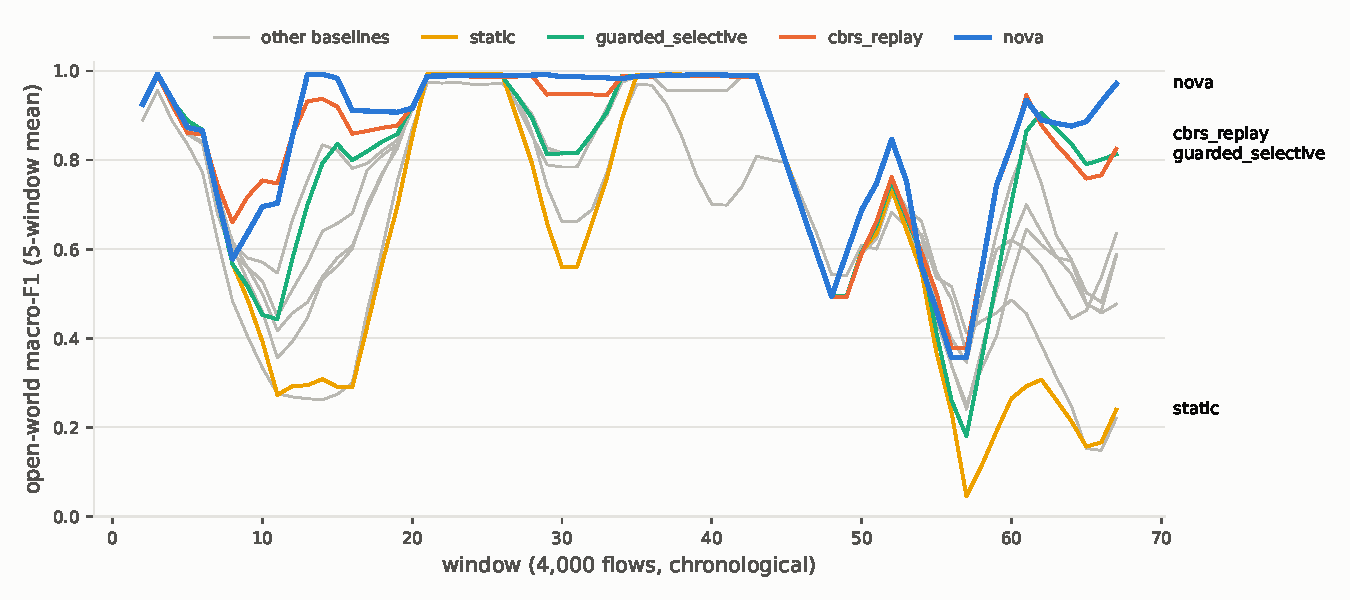
\includegraphics[width=0.78\textwidth]{fig_ow_f1_over_time_CIC17.pdf}}{\TBD{figure}}\\[2pt]
{\small (a) CIC-IDS2017}\\[6pt]
\IfFileExists{\results{fig_ow_f1_over_time_IDS18.pdf}}{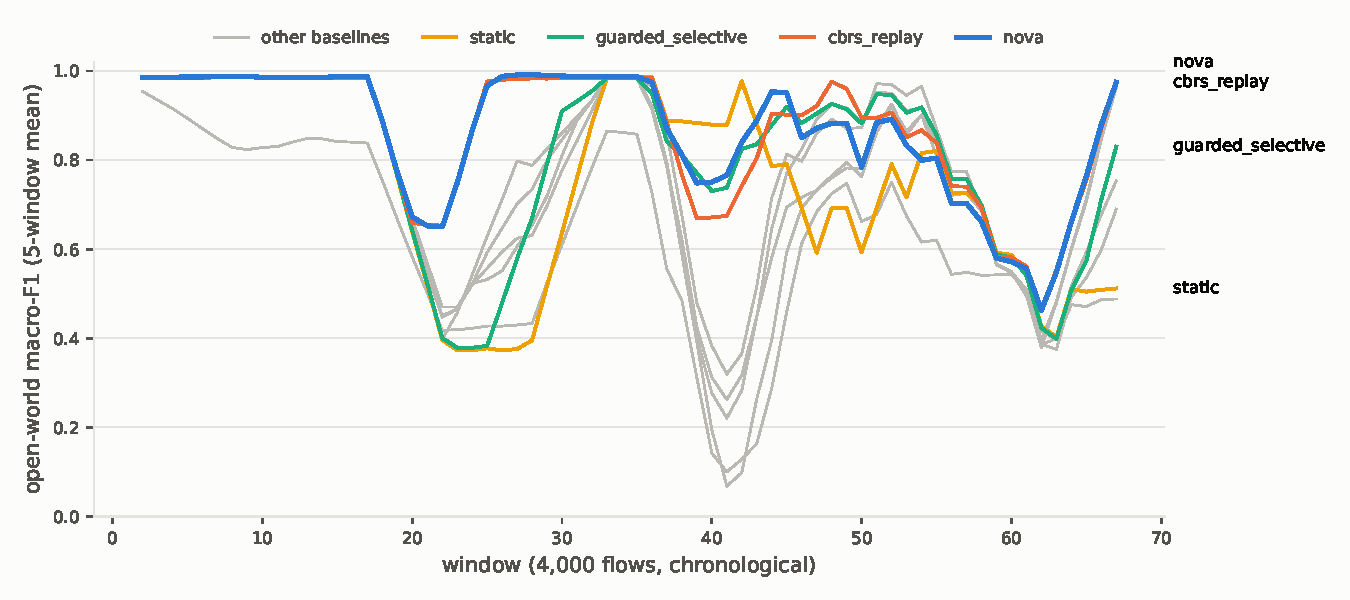
\includegraphics[width=0.78\textwidth]{fig_ow_f1_over_time_IDS18.pdf}}{\TBD{figure}}\\[2pt]
{\small (b) CSE-CIC-IDS2018}\\[6pt]
\IfFileExists{\results{fig_ow_f1_over_time_UNSW.pdf}}{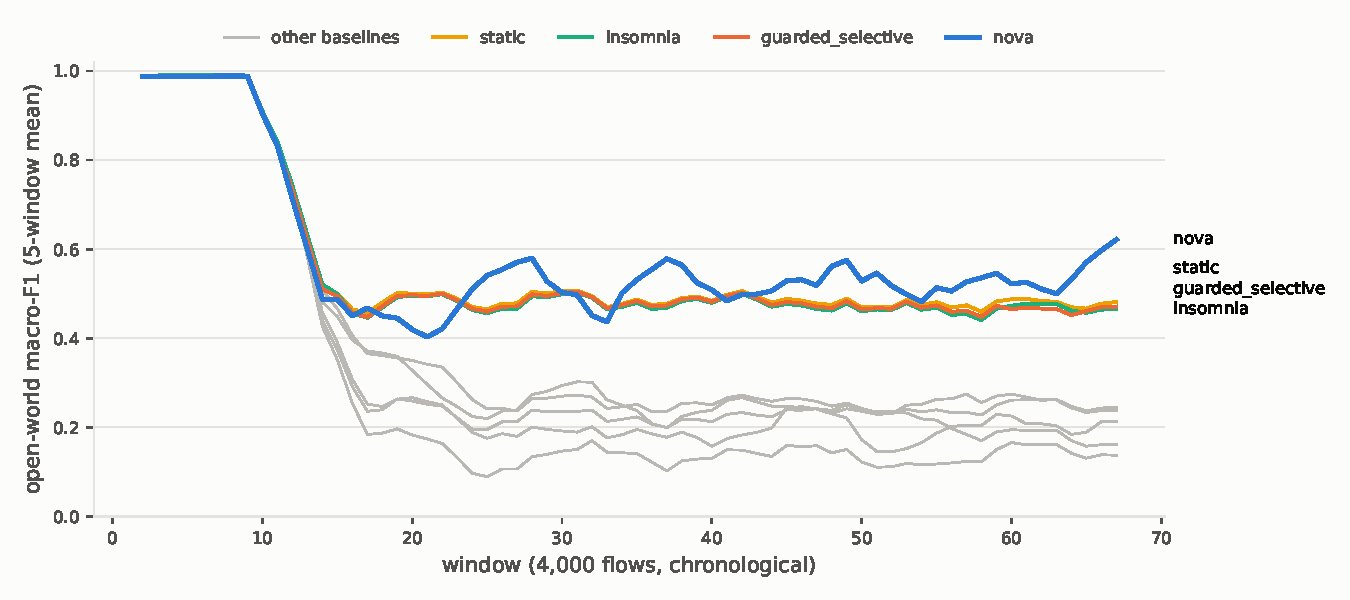
\includegraphics[width=0.78\textwidth]{fig_ow_f1_over_time_UNSW.pdf}}{\TBD{figure}}\\[2pt]
{\small (c) UNSW-NB15}
\caption{Open-world macro-F1 per window (mean of five seeds, 5-window moving average). \nova{}, the strongest
baselines and the static model are in colour; the remaining baselines are grey.}
\label{fig:time}
\end{figure}

\textbf{CIC-IDS2017} (\cref{tab:cic17}, \cref{fig:time}a). \nova{} and CBRS replay tie on OW-F1 (0.752 against
0.755). \nova{} has the higher AUT (0.860 against 0.837) and is better in 52 of the 70 windows, but the per-window
difference is within the bootstrap uncertainty ($+2.2$ points, 95\% CI $[-0.3, +4.6]$, \cref{tab:boot}). \nova{}
also varies more across seeds (0.721 to 0.776, against 0.752 to 0.757 for CBRS replay); in the two lower seeds it
names DoS GoldenEye and SQL injection less well. \nova{} is significantly ahead of every other method, by 7.0 to
23.1 points. CBRS detects slightly more attacks (detection F1 0.863 against 0.858, unknown AUROC 0.884 against
0.868), but \nova{} flags significantly fewer benign flows (2.8\% against 4.5\% pooled; per-window difference
$-4.2$ points, CI $[-9.0, -0.4]$): it sends 38\% fewer benign flows to the analyst.
The static model, which never sees a label, ends at 0.316 because every attack class in the stream is new to it.
\Cref{fig:time}a shows the shape of the stream: each attack day opens with a dip, while the new class is unknown
and partly missed, and the adaptive methods recover once labels arrive; \nova{} is on or near the top after most dips.

\textbf{CSE-CIC-IDS2018} (\cref{tab:ids18}, \cref{fig:time}b). \nova{} and CBRS replay tie on OW-F1 (0.738 against
0.730) and AUT (0.867 against 0.870). \nova{} is better in 50 of the 70 windows, but CBRS is ahead by three points
on average over the last 24 windows, the per-window difference is close to zero ($-0.4$, CI $[-2.3, +1.4]$), and
\nova{} varies more across seeds (0.655 to 0.793). On the other metrics \nova{} is ahead: detection F1 0.803 against
0.784, a significantly lower false-positive rate (3.2\% against 4.7\%; CI $[-5.5, -0.4]$), and maximum forgetting
0.008 against 0.032. Guarded selective retraining has the lowest false-positive rate on this dataset (2.7\%), but
it detects far fewer attacks (detection F1 0.592).

\textbf{UNSW-NB15} (\cref{tab:unsw}, \cref{fig:time}c). Here most adaptive methods end \emph{below} the static
model (0.499): CBRS replay reaches 0.326, continual replay 0.352 and uncertainty sampling 0.241. The per-flow
predictions show why. These methods learn Exploits and Fuzzers, but every flow of these classes is then rejected
as \unk{} (\cref{sec:res-perclass}). The open-world thresholds were calibrated on the January reference set, and
the February traffic of the same classes lies outside them. Classes that the model has learned are no longer
credited for \unk{}, so the rejections count as errors.

\nova{} recalibrates each learned class on recent labelled flows that it did not train on (the calibration store)
and reaches 0.511 OW-F1 and 0.596 AUT. This is significantly ahead of every replay-based method ($+19.6$ to
$+29.4$ points) and of guarded selective retraining ($+3.4$, CI $[+0.5, +5.8]$), and level with the static model
($+2.7$, CI $[-0.0, +4.9]$). It also has the highest detection F1 (0.858) and the lowest false-positive rate
(6.7\% against 7.5--19.0\%). Every method flags all UNSW-NB15 attack flows (detection recall 1.0), so on this
dataset the methods differ in false positives and in naming the attack class, not in missed attacks.

\textbf{Self-training.} INSOMNIA, which labels half of each window with its own nearest-centroid estimator, has
the highest false-positive rate on both CIC datasets (12.4\% and 25.8\%) and the largest forgetting on
CSE-CIC-IDS2018 (0.142). Its estimator can only assign classes that existed at training time, so flows of new
attacks are fed back into training under wrong labels.

\begin{table}[t]
\centering
\caption{Per-window difference \nova{} minus method, in points, with 95\% moving-block bootstrap intervals. OW-F1 at
budgets 10\% and 1\% (positive: \nova{} better), and false-positive rate at 10\% (negative: \nova{} flags fewer
benign flows). Intervals that exclude zero are significant.}
\label{tab:boot}
\small
\setlength{\tabcolsep}{3pt}
\loadrows{\bootA}{bootstrap_paper.tex}{4}\loadrows{\bootB}{bootstrap_b001_paper.tex}{4}%
\loadrows{\bootC}{bootstrap_fpr_paper.tex}{4}%
\resizebox{\textwidth}{!}{%
\begin{tabular}{@{}lccc@{}}
\toprule
Method & CIC-IDS2017 & CSE-CIC-IDS2018 & UNSW-NB15 \\
\midrule
\multicolumn{4}{@{}l}{\emph{OW-F1, budget 10\%}} \\
\bootA
\midrule
\multicolumn{4}{@{}l}{\emph{OW-F1, budget 1\%}} \\
\bootB
\midrule
\multicolumn{4}{@{}l}{\emph{False-positive rate, budget 10\%}} \\
\bootC
\bottomrule
\end{tabular}}
\end{table}

\textbf{Answer to RQ2.} At a 10\% budget, \nova{} ties with the strongest baseline, CBRS replay, on both CIC
datasets (stream-level differences of $-0.3$ and $+0.8$ points; per-window differences within the bootstrap
uncertainty, \cref{tab:boot}) and has the highest OW-F1 on UNSW-NB15. What is robust is the false-positive rate: \nova{} flags significantly
fewer benign flows than CBRS replay on all three datasets. The largest accuracy gap, on UNSW-NB15, comes from
recalibration; \cref{sec:res-ablation} confirms this.

\subsection{RQ3: ten times fewer labels}
\label{sec:res-budget}
\Cref{tab:budget} repeats the comparison with 1\% of each window labelled (40 flows per window) and an unchanged
configuration. The two label-free methods are omitted, because their results do not depend on the budget.

\begin{table}[t]
\centering
\caption{Label budget 1\%: OW macro-F1 and false-positive rate (\%), mean over five seeds; best per column in
bold.}
\label{tab:budget}
\small
\setlength{\tabcolsep}{4pt}
\IfFileExists{\results{budget_b001_paper.tex}}{%
\CatchFileDef{\budgetrows}{\results{budget_b001_paper.tex}}{}%
\begin{tabular}{@{}lcccccc@{}}
\toprule
\budgetrows
\bottomrule
\end{tabular}}{\TBD{budget table not generated yet}}
\end{table}

On CIC-IDS2017, where the two methods tie at 10\%, \nova{} leads CBRS replay at 1\% by 8.5 OW-F1 points (0.651
against 0.566) and 5.7 AUT points (0.818 against 0.761). \nova{} loses 0.101 OW-F1 when the budget shrinks
tenfold, CBRS replay 0.189. Unknown AUROC stays at 0.869 for \nova{} but falls to 0.787 for CBRS replay. The
per-window lead over CBRS replay is significant ($+5.7$ points, CI $[+1.4, +10.2]$). On CSE-CIC-IDS2018, \nova{}
is slightly ahead at 1\% (0.559 against 0.541; AUT 0.825 against 0.808), but the interval includes zero ($+1.5$,
CI $[-0.0, +4.7]$).

On UNSW-NB15, \nova{} is behind at 1\%: 0.470 against 0.501 for periodic retraining, significantly so per window
($-5.0$, CI $[-10.3, -0.9]$), and 0.478 for continual replay and guarded selective retraining (not significant). The per-class results show that this lead comes from \emph{not} learning. With
40 labels per window, periodic retraining never collects the five labels per class it needs to learn the four
held-out classes: in all five seeds its last model knows none of them. It keeps rejecting these classes as \unk{}, which the metric credits in full
(per-class F1 0.90 to 1.00), while it scores 0 on Exploits and Fuzzers, like the static model.

\nova{} spends its labels on novel flows, so it does learn DoS and Reconnaissance. In UNSW-NB15, however, these
overlap heavily with Exploits; in the first seed, 38\% of the DoS flows scored after DoS was learned are labelled
Exploits. A class that is learned but confused scores lower than a class that stays \unk{}. At the same time,
\nova{} has by far the lowest false-positive rate (10.7\% against 16.2--18.5\%) and the highest detection F1 (0.793
against at most 0.715).

\textbf{Answer to RQ3.} When labels are scarce, \nova{} pulls ahead on both CIC datasets, significantly on
CIC-IDS2017; the ablation of
\cref{sec:res-ablation} suggests that the query, which mainly improves unknown detection, contributes to this,
although we did not repeat the ablation at 1\%. The UNSW-NB15 result is a limit of open-world scoring, not of the query: open-world macro-F1 rewards
leaving an inseparable class unknown over learning it. Operators who prefer the second outcome should read
OW-F1 together with per-class results.

\subsection{Decomposing the open-world score}
\label{sec:res-decomp}
Because open-world macro-F1 merges two different outcomes, ``the class is unknown and rejected'' and ``the class
is known and named correctly'', \cref{tab:decomp} reports them separately from the per-flow predictions. Each flow
is either of a class known to the model that scored it, or of a class unknown to it. On known-class flows we
report macro-F1 (with \unk{} counted as an error), the share wrongly rejected as \unk{}, and the share of known
\emph{attack} flows named with their correct class. On unknown-class flows we report the share rejected as \unk{}
(unknown recall). Among all \unk{} decisions we report the share that are indeed of an unknown class (unknown
precision).

\begin{table}[t]
\centering
\caption{Open-world outcomes separated (mean over five seeds). Known: flows of classes the deployed model knows;
unknown: flows of classes it does not know.}
\label{tab:decomp}
\small
\setlength{\tabcolsep}{4pt}
\loadrows{\decA}{owparts_CIC17_b010_paper.tex}{6}\loadrows{\decB}{owparts_IDS18_b010_paper.tex}{6}%
\loadrows{\decC}{owparts_UNSW_b010_paper.tex}{6}\loadrows{\decD}{owparts_UNSW_b001_paper.tex}{6}%
\resizebox{\textwidth}{!}{%
\begin{tabular}{@{}lccccc@{}}
\toprule
 & \multicolumn{3}{c}{Known-class flows} & \multicolumn{2}{c}{Unknown-class flows} \\
\cmidrule(lr){2-4}\cmidrule(l){5-6}
Method & Macro-F1 & Falsely rejected (\%) & Attacks named correctly & Recall & Precision \\
\midrule
\multicolumn{6}{@{}l}{\emph{CIC-IDS2017, budget 10\%}} \\
\decA
\midrule
\multicolumn{6}{@{}l}{\emph{CSE-CIC-IDS2018, budget 10\%}} \\
\decB
\midrule
\multicolumn{6}{@{}l}{\emph{UNSW-NB15, budget 10\%}} \\
\decC
\midrule
\multicolumn{6}{@{}l}{\emph{UNSW-NB15, budget 1\%}} \\
\decD
\bottomrule
\end{tabular}}
\end{table}

The decomposition separates the methods more clearly than OW-F1 does. On UNSW-NB15 at 1\%, periodic retraining,
which won on OW-F1, reaches a known-class macro-F1 of only 0.150 and names 6\% of known attack flows correctly;
\nova{} reaches 0.390 and 62\%. Its OW-F1 lead therefore comes entirely from the \unk{} credit for classes it
never learns. At 10\%, \nova{}'s known-class macro-F1 on UNSW-NB15 is 0.505 against at most 0.165, and it wrongly
rejects 5.5\% of known flows against 13.4--31.1\% for the other methods, which is the stale-threshold failure in
numbers.

The decomposition also shows where \nova{} is weaker. On CSE-CIC-IDS2018, CBRS replay has the higher known-class
macro-F1 (0.781 against 0.744) and rejects more unknown flows (recall 0.668 against 0.554). \nova{}'s advantage there
is the precision of its \unk{} decisions (0.415 against 0.317), i.e.\ fewer benign or known flows sent to the
analyst as unknown. On CIC-IDS2017, \nova{} has the higher known-class macro-F1 (0.782 against 0.574) and attack
identification (0.755 against 0.667), while CBRS again rejects more unknown flows (0.614 against 0.438). Unknown
precision is low for every method on UNSW-NB15 (at most 0.10), because unknown-class flows are rare there and
most \unk{} decisions concern drifted benign traffic.

\subsection{RQ4: which components matter}
\label{sec:res-ablation}
\Cref{tab:ablation} removes one component at a time on all three datasets, and \cref{tab:ablation-ci} gives the
per-window differences with block-bootstrap intervals. The CIC-IDS2017 ablation was part of the development. The
two held-out ablations were run after the main results, with the method unchanged. The ablations use three seeds,
and full \nova{} is taken from the same three seeds of the main comparison.

The two views can disagree. Stream-level OW-F1 gives every class the same weight, so a class with a few dozen
flows counts as much as all benign traffic. The per-window difference gives every window the same weight, so a
component that matters only for a short-lived class barely moves it.

\begin{table}[t]
\centering
\caption{Ablation: stream-level OW macro-F1 (change against full \nova{} in points) and false-positive rate (\%)
with one component removed; budget 10\%, mean over three seeds. Full \nova{} is the mean over the same three seeds,
so it can differ slightly from \cref{tab:cic17,tab:ids18,tab:unsw}.}
\label{tab:ablation}
\small
\setlength{\tabcolsep}{4pt}
\IfFileExists{\results{ablation_all_paper.tex}}{%
\CatchFileDef{\ablrows}{\results{ablation_all_paper.tex}}{}%
\resizebox{\textwidth}{!}{%
\begin{tabular}{@{}lcccccc@{}}
\toprule
 & \multicolumn{2}{c}{CIC-IDS2017} & \multicolumn{2}{c}{CSE-CIC-IDS2018} & \multicolumn{2}{c}{UNSW-NB15} \\
Variant & OW-F1 & FPR & OW-F1 & FPR & OW-F1 & FPR \\
\midrule
\ablrows
\bottomrule
\end{tabular}}}{\TBD{ablation table not generated yet}}
\end{table}

\begin{table}[t]
\centering
\caption{Ablation, per window: mean difference ablated minus full \nova{} over the 70 windows (points, both
averaged over the same three seeds), with 95\% moving-block bootstrap intervals. Negative OW-F1 and positive FPR
differences mean that the component helps.}
\label{tab:ablation-ci}
\small
\setlength{\tabcolsep}{4pt}
\loadrows{\ablciA}{bootstrap_ablation_paper.tex}{4}%
\loadrows{\ablciB}{bootstrap_ablation_fpr_paper.tex}{4}%
\resizebox{\textwidth}{!}{%
\begin{tabular}{@{}lccc@{}}
\toprule
Variant & CIC-IDS2017 & CSE-CIC-IDS2018 & UNSW-NB15 \\
\midrule
\multicolumn{4}{@{}l}{\emph{OW macro-F1}} \\
\ablciA
\midrule
\multicolumn{4}{@{}l}{\emph{False-positive rate}} \\
\ablciB
\bottomrule
\end{tabular}}
\end{table}

\textbf{CIC-IDS2017.} Removing any component lowers stream-level OW-F1, by 1.2 to 5.6 points. For the guard, the
query, recency weighting and the balanced memory the drop occurs in every seed; for the calibration store and
propagation its sign varies between seeds. Per window, no difference is significant on its own; the query and
the calibration store come closest ($-1.1$ each, upper bound 0.0). The guard has the largest stream-level effect
($-5.6$; $-5.3$ to $-5.9$ in the three seeds), and it is concentrated in two classes. Without the guard, XSS falls
from 0.98 to 0.40 F1, mostly because \nova{} deploys models that name its flows Brute Force, and Bot falls from 0.24
to 0.01, because a deployed model knows the class but rejects its flows. With the guard, the candidates that
confuse the two web attacks are rejected and XSS flows stay \unk{}, which open-world macro-F1 credits in full. Part
of the guard's benefit on CIC-IDS2017 is therefore the credit for not learning a class that cannot be learned well
from a few labels (\cref{sec:discussion}). Without the hold-out check, more updates are deployed. They flag more
attack flows (detection recall 0.836 against 0.799) but name the right class less often (open-world attack
macro-recall 0.640 against 0.685), and binary detection does not penalise naming the wrong class. The query mainly
improves unknown detection (unknown AUROC 0.826 without it, against 0.872), and propagation keeps the
false-positive rate down (3.6\% without it, against 2.8\%).

\textbf{UNSW-NB15.} Here the guard and the calibration store are essential. Without the guard, stream-level OW-F1
falls by 22 points in every seed (per window $-24.9$, CI $[-31.1, -18.4]$); without the calibration store, by 6 to
14 points ($-17.7$ per window). Both variants fail in the same way: Exploits and Fuzzers drop to zero F1, the
stale-threshold failure of the replay baselines (\cref{sec:res-main}). The calibration store prevents it by
recalibrating learned classes; the guard prevents it by not deploying candidates that lose on the newest labelled
window. The query ($-4.2$) and the balanced memory ($-4.0$) also help significantly per window. Recency weighting and
propagation slightly lower OW-F1 ($+0.5$ each when removed; the intervals just exclude or touch zero), but
propagation lowers the false-positive rate significantly ($+1.5$ points without it).

\textbf{CSE-CIC-IDS2018.} The stream-level differences are large but inconsistent. Removing the guard changes OW-F1
by $+13.7$, $-3.5$ and $+4.8$ points in the three seeds, and the other components vary similarly. The reason is the
composition of the stream (\cref{tab:audit}): four of its nine classes have 33, 14, 7 and 2 flows, and each
counts one ninth of macro-F1. Full \nova{} scores 0.54 on LOIC-UDP (33 flows), where four of the six ablated
variants score 1.00; this single class accounts for about five points of OW-F1. Per window, only the query
($-1.5$, CI $[-3.1, -0.3]$) and propagation ($-1.8$, CI $[-3.6, -0.5]$) have a significant effect, and both help.
Removing the guard makes no significant difference to OW-F1, but it raises the false-positive rate ($+1.5$ points,
CI $[+0.1, +4.3]$).

In short, removing the query, the calibration store or the guard lowers per-window OW-F1 on all three datasets,
but only the query does so significantly on both held-out datasets. The guard and the calibration store are what
keep \nova{} working on UNSW-NB15; elsewhere they mainly affect a few short-lived classes and the false-positive
rate. Recency weighting and propagation do not help OW-F1 on UNSW-NB15.

\textbf{What the guard does.} \Cref{tab:guard} counts the guard's decisions. In each run, \nova{} proposes one
candidate per labelled window (69). At a 10\% budget, the guard rejects 17 to 24 of them and rolls back a deployed
model three to eight times on average. Every rejection is due to the hold-out comparison; the reference-forgetting
check never fired, so in these streams it acts only as a safety net. A share of the rejected candidates (5.4 to 7.4
of 17 to 19 on the CIC datasets) had learned a class the deployed model did not know. This reveals a bias of comparing models
with open-world credit: the deployed model receives full credit for rejecting a class it does not know, while the
candidate is scored on how well it names that class, so a candidate that learns a new class imperfectly can lose
the comparison. The guard is therefore conservative towards new classes. At a 1\% budget the hold-out holds only
about ten labelled flows (minimum 8 to 9), so the guard's decisions rest on very little evidence. The ablation
shows that the guard helps at 10\% on UNSW-NB15 and, at stream level, on CIC-IDS2017, but we did not test whether
it helps or hurts at 1\%.

\begin{table}[t]
\centering
\caption{Deployment-guard decisions per \nova{} run (mean over five seeds; 69 candidates per run).}
\label{tab:guard}
\small
\setlength{\tabcolsep}{3pt}
\IfFileExists{\results{guard_paper.tex}}{%
\CatchFileDef{\guardrows}{\results{guard_paper.tex}}{}%
\resizebox{\textwidth}{!}{%
\begin{tabular}{@{}llcccccccc@{}}
\toprule
 & & & & \multicolumn{4}{c}{Rejected} & & \\
\cmidrule(lr){5-8}
Dataset & Budget & Proposed & Deployed & All & Hold-out loss & Forgetting & With new class & Rollbacks &
Hold-out size, median (min) \\
\midrule
\guardrows
\bottomrule
\end{tabular}}}{\TBD{guard table not generated yet}}
\end{table}

\textbf{Open-world detector.} Replacing the class-conditional $k$-NN detector by the distance to the nearest class
centroid (three seeds, compared with the same seeds of the main comparison) lowers OW-F1 on CIC-IDS2017 from 0.311
to 0.178 for the static model and from 0.768 to 0.712 for \nova{}.
Unknown AUROC drops from 0.605 to 0.520 and from 0.872 to 0.840. With the centroid detector, the static model
labels almost every attack as benign (detection F1 0.012). A plausible explanation is that benign traffic
consists of many modes: its centroid lies between them, its distance scale becomes large, and attack flows fall
inside it. The $k$-NN
detector is therefore useful even without adaptation, and every method in \cref{tab:cic17,tab:ids18,tab:unsw} uses
it.

\subsection{RQ5: sensitivity to delay, thresholds and classifier}
\label{sec:res-sens}
\textbf{Label delay.} \Cref{tab:delay} varies the delay on CIC-IDS2017 for \nova{} and CBRS replay (three seeds;
the delay-1 columns are the same three seeds of the main comparison). AUT falls with the delay for both methods,
from 0.899 to 0.806 for \nova{} and from 0.854 to 0.803 for CBRS replay, because every new class is rejected or
misnamed for longer. Stream-level OW-F1 does not fall monotonically: at delay 0 it is lower than at delay 1 for
both methods. Without delay, most classes are learned earlier and improve (PortScan from 0.49 to 0.80 for
\nova{}), but the short-lived web attacks are learned from their first few labels and confused with each other
(\nova{}'s XSS F1 falls from 0.98 to 0.14), whereas with a one-window delay they stay \unk{} and receive full
open-world credit. \nova{}'s per-window lead over CBRS replay shrinks with the delay: $+4.5$ points at delay 0 (CI
$[+1.7, +7.7]$), $+2.0$ at delay 1 (CI $[-0.5, +4.3]$) and $+0.3$ at delay 3 (CI $[-1.9, +2.0]$). Its false-positive
rate stays significantly lower at every delay (2.5, 2.8 and 3.4\% against 4.4, 4.5 and 4.5\%). The quicker the
labels arrive, the more \nova{}'s choice of what to label matters; with a three-window delay the two methods are
equally accurate.

\begin{table}[t]
\centering
\caption{Label delay on CIC-IDS2017 (budget 10\%): OW-F1, AUT and FPR (\%), mean over three seeds.}
\label{tab:delay}
\small
\IfFileExists{\results{delay_paper.tex}}{%
\CatchFileDef{\delayrows}{\results{delay_paper.tex}}{}%
\resizebox{\textwidth}{!}{%
\begin{tabular}{@{}lccccccccc@{}}
\toprule
 & \multicolumn{3}{c}{Delay 0} & \multicolumn{3}{c}{Delay 1 (main)} & \multicolumn{3}{c}{Delay 3} \\
Method & OW-F1 & AUT & FPR & OW-F1 & AUT & FPR & OW-F1 & AUT & FPR \\
\midrule
\delayrows
\bottomrule
\end{tabular}}}{\TBD{delay table not generated yet}}
\end{table}

\textbf{Rejection thresholds.} The quantiles of \cref{sec:unknown} set how many flows are sent to the analyst.
\Cref{tab:review} shows a stricter setting (1\% and 99.5\%) and a more lenient one (5\% and 97\%) besides the
default (2\% and 99\%), with three seeds. Lenient thresholds raise OW-F1 for every method (\nova{} 0.791, CBRS
replay 0.784, static 0.423), because more flows of new classes are rejected and credited, but they more than double
the review load (\nova{} from 2.8\% to 6.9\% of benign flows, CBRS replay from 4.5\% to 9.3\%). Strict thresholds
nearly halve \nova{}'s false-positive rate (1.5\%) but cost it ten OW-F1 points (0.671), more than CBRS replay
loses (0.727). At every setting \nova{} flags fewer benign flows than CBRS replay (1.5, 2.8 and 6.9\% against 2.5,
4.5 and 9.3\%). At a similar review load, \nova{} with default thresholds (2.8\%) reaches 0.768 against 0.727 for
CBRS replay with strict ones (2.5\%). The thresholds therefore move every method along a trade-off between review
load and OW-F1 rather than change their order, and they should be set from the analysts' capacity.

\begin{table}[t]
\centering
\caption{Rejection thresholds on CIC-IDS2017 (budget 10\%): stricter = MSP 1\%, $k$-NN 99.5\%; default = 2\%,
99\%; more lenient = 5\%, 97\%. Mean over three seeds (default: the same three seeds of the main comparison);
FPR in \%.}
\label{tab:review}
\small
\IfFileExists{\results{review_paper.tex}}{%
\CatchFileDef{\reviewrows}{\results{review_paper.tex}}{}%
\begin{tabular}{@{}llcccc@{}}
\toprule
Method & Thresholds & OW-F1 & Detection recall & FPR & U-AUROC \\
\midrule
\reviewrows
\bottomrule
\end{tabular}}{\TBD{review table not generated yet}}
\end{table}

\textbf{Neural classifier.} \Cref{tab:mlp} replaces gradient boosting by a two-layer MLP (128 and 64 units, 25
epochs) for the three most informative methods. \nova{} keeps the lowest false-positive rate (3.3\% against 4.7\%
for CBRS replay) and the highest detection F1 (0.865 against 0.824), both methods have the same AUT (0.831 against
0.833), and \nova{} is better in 49 of 70 windows. Its stream-level OW-F1, however, is clearly lower (0.622 against
0.711). Per-class F1 shows why: the two methods differ mostly on short-lived web attacks, XSS (0.09 against 0.68)
and Brute Force (0.28 against 0.47). Each appears in only a few windows, so they move the per-window curve little but
carry a full class weight in macro-F1. In our implementation, recency weighting is not applied to the MLP, which
takes no sample weights. We therefore do not claim that \nova{}'s accuracy advantage carries over to neural
classifiers; its lower false-positive rate does. Interestingly, the static MLP has a much higher unknown AUROC
than the static gradient-boosting model (0.915 against 0.608), which suggests that the open-world score depends on
the representation; we return to this in \cref{sec:res-meta}.

\resulttable[t]{CIC17_model-mlp_b010_paper.tex}{CIC-IDS2017 with an MLP classifier (budget 10\%, three seeds).}{tab:mlp}

\subsection{Per-class results and failure modes}
\label{sec:res-perclass}
\Cref{tab:perclass-cic,tab:perclass-ids,tab:perclass-unsw} list per-class open-world F1 for \nova{}, the
strongest baseline, guarded selective retraining and the static model.

\newcommand{\perclasstable}[3]{%
\begin{table}[t]
\centering
\caption{#2: per-class open-world F1 (budget 10\%, mean over five seeds). ``New'': unknown to the initial
model. Best per row in bold.}
\label{#3}
\small
\IfFileExists{\results{#1}}{%
\CatchFileDef{\pcrows}{\results{#1}}{}%
\begin{tabular}{@{}lrccccc@{}}
\toprule
Class & Stream flows & New & \nova{} & CBRS replay & Guarded sel. & Static \\
\midrule
\pcrows
\bottomrule
\end{tabular}}{\TBD{per-class table not generated yet}}
\end{table}}
\perclasstable{perclass_CIC17_paper.tex}{CIC-IDS2017}{tab:perclass-cic}
\perclasstable{perclass_IDS18_paper.tex}{CSE-CIC-IDS2018}{tab:perclass-ids}
\perclasstable{perclass_UNSW_paper.tex}{UNSW-NB15}{tab:perclass-unsw}

On CIC-IDS2017, \nova{} reaches 0.82--1.00 on nine of the thirteen classes. Four classes cap every method:
PortScan, DoS slowloris, SSH-Patator and Bot. They fail for different reasons. SSH-Patator occurs only in the first
window of the stream and DoS slowloris in two early windows. No adaptive method can learn them under a one-window
delay, so their F1 depends only on whether the initial model rejects them. Most of their flows are predicted
benign. In the first seed, the $k$-NN distance separates slowloris flows from benign ones well (AUROC 0.97 among
flows predicted benign), but at the benign threshold only about a fifth are rejected. After being learned,
PortScan is still confused with benign traffic in about a third of its flows (first seed), consistent with the feature-identical port-scan and
benign flows reported for this dataset~\cite{engelen2021troubleshooting}. Bot is the only class where \nova{} is
clearly better than every baseline (0.24 against 0.01); the others never learn it.

On UNSW-NB15 (\cref{tab:perclass-unsw}), CBRS replay scores 0 on Exploits, Fuzzers, Analysis and Backdoor
and 0.54 on Generic, whereas \nova{} reaches 0.65, 0.55, 0.09, 0.06 and 0.97. This is the recalibration effect of
\cref{sec:res-main} at the class level. Conversely, the static model and guarded selective retraining score 0.99
to 1.00 on the held-out DoS, Reconnaissance and Shellcode, because they keep rejecting them, while \nova{} learns
them imperfectly (0.38--0.75).

On CSE-CIC-IDS2018 (\cref{tab:perclass-ids}), \nova{} and CBRS replay are within 0.04 of each other on the four
classes with thousands of stream flows other than Infilteration. Infilteration caps every method (at most 0.16):
in the first seed, 95\% of its flows are predicted benign by \nova{} and 80\% by CBRS replay. The static model
scores 1.00 on HOIC because it rejects every HOIC flow as \unk{}. The remaining four classes have 2 to 33 stream
flows (\cref{tab:audit}). \nova{} is better on LOIC-UDP and XSS (0.72 and 0.97 against 0.43 and 0.84), CBRS replay
on Brute Force-Web and SQL injection (0.75 and 0.80 against 0.56 and 0.73). Together these four classes carry four
ninths of macro-F1, which is why the stream-level comparison on this dataset is fragile
(\cref{sec:res-ablation}).

\subsection{Would a learned representation help?}
\label{sec:res-meta}
Bot, PortScan and the early DoS attacks fail because their flows lie close to benign flows in the feature space.
A learned embedding might separate them. We tested this offline on CIC-IDS2017 only, before considering any change
to \nova{}.

At three points in the stream (windows 5, 25 and 45), we took the labelled pool that a 10\%-budget method would
have, and trained an MLP encoder (two hidden layers of 256 units, 64-dimensional normalised output) on the GPU in
two ways. The first uses class-balanced prototypical episodes~\cite{snell2017prototypical}. The second uses the same
episodes plus one known class held out per episode as a pseudo-unknown, pushed away from all prototypes by a
margin; this is open-set meta-learning in the style of PEELER~\cite{liu2020peeler}. We then measured how well the
$k$-NN distance to benign flows separates future unseen attacks from benign flows of the same period. Thresholds
were set on held-out benign flows of the pool, never on the future. \Cref{tab:meta} shows the second cut point.

\begin{table}[t]
\centering
\caption{Representation-learning probe on CIC-IDS2017, cut at window 25 (pool: benign, FTP-Patator, SSH-Patator
and four DoS classes). Detection rate of future unseen attack classes at the threshold that gives a 1\% benign
false-positive rate on held-out pool flows, and the false-positive rate that threshold actually produces on
future benign traffic.}
\label{tab:meta}
\small
\begin{tabular}{@{}lccc@{}}
\toprule
 & Raw features & Prototypical & Open-set meta-learning \\
\midrule
Realised benign FPR (target 1\%) & 3.1\% & 0.8\% & 0.7\% \\
\midrule
DDoS & 0.16 & 0.66 & 0.70 \\
Web Attack -- SQL injection & 0.00 & 0.67 & 0.67 \\
Web Attack -- Brute Force & 0.00 & 0.14 & 0.14 \\
Web Attack -- XSS & 0.00 & 0.03 & 0.03 \\
Infiltration & 1.00 & 0.00 & 0.00 \\
PortScan & 0.00 & 0.01 & 0.01 \\
Bot & 0.00 & 0.00 & 0.00 \\
\bottomrule
\end{tabular}
\end{table}

Both embeddings keep the benign false-positive rate close to its target on later traffic. They raise the detection
rate for DDoS and SQL injection, but lose Infiltration. The open-set episodes bring no consistent gain over plain
prototypical training, at this cut point or the other two. At the 1\% threshold, Bot, PortScan and XSS stay below
5\% detection in every representation and at every cut point. The remaining errors on these classes therefore reflect overlap with benign
traffic in the flow features, not a lack of model capacity, and we did not add the embedding to \nova{}. The
better-calibrated false-positive rate of the embeddings is worth pursuing, but it would have to be combined with
the raw-feature detector to keep classes such as Infiltration.

\subsection{Cost}
\label{sec:res-cost}
\Cref{tab:cost} lists the total training time per 70-window run. \nova{} trains once per window on the memory plus
new labels and spends 12 to 14 minutes per run, compared with 7 to 12 minutes for CBRS replay. Prediction
including the $k$-NN score takes about 0.05\,ms per flow on a CPU when a window is scored as a batch. Labels are identical for all
label-using methods by construction.

\begin{table}[t]
\centering
\caption{Total training time per run in minutes (budget 10\%, mean over five seeds; 16-core CPU).}
\label{tab:cost}
\small
\IfFileExists{\results{cost_paper.tex}}{%
\CatchFileDef{\costrows}{\results{cost_paper.tex}}{}%
\begin{tabular}{@{}lccc@{}}
\toprule
Method & CIC-IDS2017 & CSE-CIC-IDS2018 & UNSW-NB15 \\
\midrule
\costrows
\bottomrule
\end{tabular}}{\TBD{cost table not generated yet}}
\end{table}

\section{Discussion}
\label{sec:discussion}

\subsection{Implications for practice}
\textbf{Stale thresholds are a silent failure.} The most consequential result is not the ranking of the methods
but the UNSW-NB15 failure of the replay baselines (\cref{sec:res-main,sec:res-ablation}). These methods learn the
right classes from the right labels, yet every later flow of those classes is rejected, because the rejection
thresholds were fitted on older traffic. The failure is invisible in the classifier's training loss and in its
detection recall, which stays at 1.0. Any open-world detector whose thresholds are calibrated once is exposed to
it. The remedy is cheap: keep a small store of held-out analyst labels per class and recalibrate on it whenever
the model changes.

\textbf{False positives depend on calibration as much as on the model.} Most benign flows flagged by any method are
\unk{} decisions, not attack labels. Their number is set largely by the rejection quantiles, which all methods
share. A 2.8\% review rate is still large in absolute terms: at one million benign flows a day it means about
28{,}000 reviews, an instance of the base-rate fallacy~\cite{arp2022dos}. \Cref{sec:res-sens} shows how the
quantiles trade review load against recall. Operators should set them from their review capacity, not from a
benchmark.

\textbf{Validate every update.} The deployment guard is the component whose removal costs the most on the
development dataset. A retraining loop that deploys every candidate learns more attack traffic, but it also
deploys models that confuse classes. A hold-out check on the newest labels and a forgetting check on a fixed
reference set are simple to add to any adaptation loop.

\textbf{Read open-world scores with per-class results.} Open-world macro-F1 makes methods that learn different
classes comparable, but it credits a class that is never learned and always rejected as fully correct
(\cref{sec:metrics,sec:res-budget}). A method can therefore win by not learning. We recommend reporting
per-class results and binary detection metrics alongside it, as we do.

\subsection{Threats to validity}
\textbf{Dataset errors.} CIC-IDS2017 and CSE-CIC-IDS2018 contain labelling and feature-extraction
errors~\cite{engelen2021troubleshooting,lanvin2022errors,liu2022error}. Some port-scan flows are feature-identical to
benign flows, and Brute Force and XSS are barely separable. These errors cap every method alike and probably explain
part of the PortScan and web-attack results. Several CSE-CIC-IDS2018 day files are truncated in the published CSVs.
Results on the corrected CIC-IDS2017 release are future work.

\textbf{Short time spans.} The datasets cover two to ten days, so the streams mix attack onsets with modest benign
drift; long-term drift of benign traffic is under-represented. UNSW-NB15 needs held-out classes to contain new
attacks at all.

\textbf{Re-implemented baselines.} The baselines are re-implemented in one multi-class framework with the same
classifier and labelling cost, not run from the authors' code. INSOMNIA and the active-learning baselines were
designed for binary detection or one-shot adaptation, and NetGuard's generative augmentation is not reproduced. Our
results compare the strategies under our protocol; they do not reproduce the original papers' numbers.

\textbf{Simulated analyst.} The oracle returns correct labels with a fixed delay. Real analysts make mistakes,
answer at variable speed, and prefer some flows over others. Label noise would hurt label propagation and the
guard in particular.

\textbf{Design on one dataset.} All design decisions were made on CIC-IDS2017. We checked the class composition of
the other two datasets once, with the static model, which determined the UNSW-NB15 hold-out. The held-out ablations
and the low-budget runs were added after the main results; they are analyses, not design steps.

\textbf{Statistics.} We use three seeds per configuration. The paired Wilcoxon tests treat windows as samples,
but consecutive windows are correlated, so the $p$-values overstate certainty. The seed changes sampling and
initialisation but not the data, so the reported deviations do not include data variability.

\section{Conclusion}
\label{sec:conclusion}

Random-split evaluation makes network intrusion detection look solved: the same classifier that is 99.8\% accurate
on a random split of CIC-IDS2017 loses most of its macro-F1 when it meets the future. We evaluated adaptation
strategies under the conditions of a deployment: chronological replay, attack classes that appear after training,
and a small, delayed labelling budget, with metrics that remain comparable when methods learn different classes.

\nova{} combines class-conditional open-world rejection with per-class recalibration, a novelty-weighted and
diverse query, conservative label propagation, a class-balanced memory and a guarded deployment loop. At a 10\%
budget it is the best or tied-best method on open-world macro-F1 on all three datasets, with a lower false-positive
rate than the strongest baseline on each. At a 1\% budget, it leads on both CIC datasets. Recalibrating the
rejection thresholds of learned classes on recent held-out labels is what keeps it above the never-updated model on
UNSW-NB15, where every other adaptive method falls below it.

The approach has clear limits. Short-lived attacks that resemble benign traffic remain undetected by every method
and every representation we tried, including a meta-learned embedding. The accuracy gain did not carry over to an
MLP classifier, and on one dataset at the smallest budget, open-world scoring favours methods that never learn the
new classes. Future work should evaluate with noisy analysts, longer captures and corrected datasets, and combine
learned and raw-feature detectors to gain the better-calibrated false-positive rate of the former without losing
classes such as infiltration. All runs, configurations and per-flow predictions are released to make such
comparisons cumulative.

\section*{CRediT authorship contribution statement}
\TBD{Author name}: Conceptualization, Methodology, Software, Investigation, Formal analysis, Writing -- original
draft, Writing -- review \& editing. \TBD{Add one line per co-author with their CRediT roles.}

\section*{Declaration of competing interest}
The authors declare that they have no known competing financial interests or personal relationships that could
have appeared to influence the work reported in this paper.

\section*{Data availability}
CIC-IDS2017, CSE-CIC-IDS2018 and UNSW-NB15 are publicly available from their providers. The code, experiment
configurations, analysis scripts and per-flow predictions of every run will be made available at \TBD{repository
URL / DOI}.

\section*{Declaration of generative AI and AI-assisted technologies in the writing process}
During the preparation of this work the authors used Claude (Anthropic), an AI assistant, to help implement the
experimental software, run and analyse the experiments, and draft and edit the manuscript. After using this tool,
the authors reviewed and edited the content as needed and take full responsibility for the content of the
publication.

\section*{Acknowledgements}
\TBD{Acknowledgements and funding, if any.}


\bibliographystyle{elsarticle-num}
\bibliography{refs}

\end{document}
